\FloatBarrier
\newpage

\section{\mfourt Models}
\label{sec:appendix:modeling}



Direct speech-to-text translation models 
have made significant progress in recent years \citep{Berard2016ListenAT,Weiss2017SequencetoSequenceMC,di2019must,agrawal-etal-2023-findings}, and achieved parity with cascaded models on academic benchmarks under specific situations (e.g., constrained data, in-domain settings, specific language pairs, etc.). However, with the arrival of massively multilingual translation models~\citep{nllb2022, siddhant2022towards, m2m100} and weakly supervised \asr models~\citep{whisper, google_usm, mms}, which leverage massive quantities of labeled data for training large foundation models, these comparisons have become outdated. To put it simply,  direct models now lag significantly behind strong cascaded models.

One of our goals with \mfourt is to bridge the gap between direct and cascaded models for \st in large multilingual and multimodal
settings by building a stronger direct \xt model (for translating both text and speech into text) that combines 
a strong speech representation learning model with a massively multilingual \mt model.
Beyond text outputs, our second goal builds on recent speech translation advancements, which have placed much emphasis on building systems that produce speech outputs~\citep{jia:interspeech:2019, lee-etal-2022-direct,unity}.
We enable speech-to-speech translation with \unity~\citep{unity}, a two-pass modeling framework that first generates text and subsequently predicts discrete acoustic units. 
Unlike cascaded models,
the different components in \unity (see \Cref{fig:modeling:overview}) can be jointly optimized.\footnote{There are two views of what constitutes a direct model in speech-to-speech translation literature: (1) A model that does not use intermediate text representation \citep{lee-etal-2022-direct} and (2) A model that directly predicts the target spectrogram~\citep{pmlr-v162-jia22b}}

The aforementioned approach alleviates the issue of cascaded error propagation and domain mismatch, while relying on an intermediate semantic representation to mitigate the problem of multi-modal source-target mapping.
 The vocoders for synthesizing speech are trained separately (see \Cref{sec:modeling:s2st:data}).
\begin{figure}[!htb]
\centering
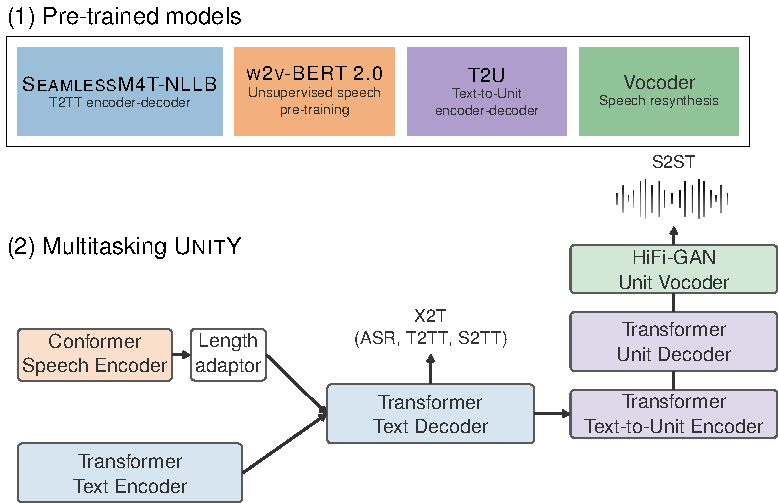
\includegraphics[width=.8\linewidth]{figures/modeling/modeling_overview_simplified.pdf}
\caption{\textbf{Overview of \mfourt.} (1) shows the pre-trained models used when finetuning multitasking \unity. (2) outlines multitasking \unity with its two encoders, text decoder, T2U encoder-decoder, and the supporting vocoders for synthesizing output speech in \sst. 
}\label{fig:modeling:overview}
\end{figure}
\Cref{fig:modeling:overview} provides an overview of the \mfourt model, including its four building blocks: 
(1) \nllbv a massively multilingual \mt model, 
(2) \wvbert, a speech representation learning model that leverages unlabeled speech audio data, 
(3) T2U, a text-to-unit sequence-to-sequence model, and 
(4) multilingual HiFi-GAN unit vocoder for synthesizing speech from units. 

The \mfourt multitask \unity model integrates components from the first three building blocks and is fine-tuned in three stages, starting from an \xt model (1,2) with English target only and ending with a full-fledged multitask \unity (1,2,3) system capable of performing \mt, \st and \sst, as well as \asr. 
In what follows, we first describe unsupervised speech pre-training (\wvbert) in \Cref{sec:modeling:x2t:w2vbert}.
We then introduce the \xt model in \Cref{sec:modeling:x2t}, starting with the data preparation pipeline in \Cref{sec:modeling:x2t:data}.
\Cref{sec:modeling:x2t:nllb} describes our multilingual \mt model, and \Cref{sec:modeling:x2t:stage12} details how the speech encoder and the \mt model are jointly fine-tuned for \xt with multimodal and multitask capabilities.
Next, we look at the \sst{} task, starting from the acoustic unit extraction pipeline and vocoder design to map units back to speech waveforms in \Cref{sec:modeling:s2st:data}
Then, we describe T2U pre-training in \Cref{sec:modeling:s2st:t2u}. 
\Cref{sec:modeling:s2st:stage3} ultimately outlines
how all these components come together in the third and final stage of fine-tuning. We evaluated our model using standard automatic metrics in \Cref{sec:modeling:main} and compared its performance with state-of-the-art speech translation models.

\subsection{Unsupervised Speech Pre-training}\label{sec:modeling:x2t:w2vbert}



Labels for speech recognition and translation tasks are scarce and expensive, especially for low-resource languages. It is challenging to train speech translation models with only limited access to supervision. 
Self-supervised pre-training with unlabeled speech audio data is, thus, a practical approach for reducing the need for supervision in model training. 
This method helps achieve the same recognition and translation quality with much less labeled data than models without pre-training. It also helps push the limits of model performance with the same amount of labeled data.
The most recent and publicly available state-of-the-art multilingual speech pre-trained model is MMS~\citep{mms}. It extends its predecessor, \xlsr~\citep{babu2021xls}, with additional 55K hours of training data and covers more than 1,300 new languages (see \Cref{tbl:modeling:sslsota}).
Besides MMS, USM~\citep{google_usm} is a proprietary SOTA multilingual speech pre-trained model that leverages the latest model architecture (BEST-RQ~\citep{best_rq} instead of wav2vec 2.0~\citep{baevski2020wav2vec}), has the largest scale of training data (12M hours), and covers more than 300 languages. 

\begin{table}[!t]
\small
    \centering
    \begin{tabular}{@{}lrrlc@{}}
        \toprule
        {\bf Model} & {\bf Languages} & {\bf Hours} & {\bf Model type} & {\bf Open model} \\
        \midrule
        \xlsrstot & 128 & 0.4M & wav2vec 2.0~\citep{baevski2020wav2vec} & $\checkmark$ \\
        USM & over $300^\dagger$ & 12M & BEST-RQ~\citep{best_rq} &  \\
        MMS & 1406 & 0.5M & wav2vec 2.0~\citep{baevski2020wav2vec} & $\checkmark$ \\
        \mfourtlg & over $\wvbertlangs^\dagger$ & 1M & \wvbert & $\checkmark$ \\
        \bottomrule
    \end{tabular}
    \caption{A comparison of multilingual speech pre-training in state-of-the-art \asr and \st models. $^\dagger$Estimated from the part of data that has language information.} 
    \label{tbl:modeling:sslsota}
\end{table}

\wvbert follows w2v-BERT~\citep{chung2021w2v} to combine contrastive learning and masked prediction learning, and improves w2v-BERT with additional codebooks in both learning objectives.
The contrastive learning module is used to learn Gumbel vector quantization (GVQ) codebooks and contextualized representations that are fed into the subsequent masked prediction learning module. The latter refines the contextualized representations by a different learning task of predicting the GVQ codes directly instead of polarizing the prediction probability of correct and incorrect codes at the masked positions. Instead of using a single GVQ codebook, \wvbert follows~\cite{baevski2020wav2vec} to use product quantization with two GVQ codebooks. Its contrastive learning loss $\mathcal{L}_c$ is the same as that in w2v-BERT, including a codebook diversity loss to encourage the uniform usage of codes. Following w2v-BERT, we use GVQ codebooks for masked prediction learning and denote the corresponding loss as $\mathcal{L}_{m_\text{GVQ}}$.
We also created an additional masked prediction task using random projection quantizers~\citep{best_rq} (RPQ), for which we denote the corresponding loss as $\mathcal{L}_{m_\text{RPQ}}$. The overall \wvbert training loss $\mathcal{L}$ is defined as follows:
\begin{align}
\mathcal{L} & = w_{c}\mathcal{L}_{c} +  w_{m_\text{GVQ}} \mathcal{L}_{m_\text{GVQ}} + 
 w_{m_\text{RPQ}} \mathcal{L}_{m_\text{RPQ}},
\end{align}
where loss weights $w_c$, $w_{m_\text{GVQ}}$ and $w_{m_\text{RPQ}}$ are set to $1.0$, $0.5$, and $0.5$, respectively. 

We follow the w2v-BERT XL architecture~\citep{chung2021w2v} for the \wvbert pre-trained speech encoder in \mfourtlg, which has 24 Conformer layers~\citep{gulati2020conformer} and approximately 600M model parameters. The \wvbert model is trained on 1 million hours of open speech audio data that covers over 143 languages.


\subsection{\xt: Into-Text Translation and Transcription}\label{sec:modeling:x2t}
\begin{figure}[!htb]
    \centering
    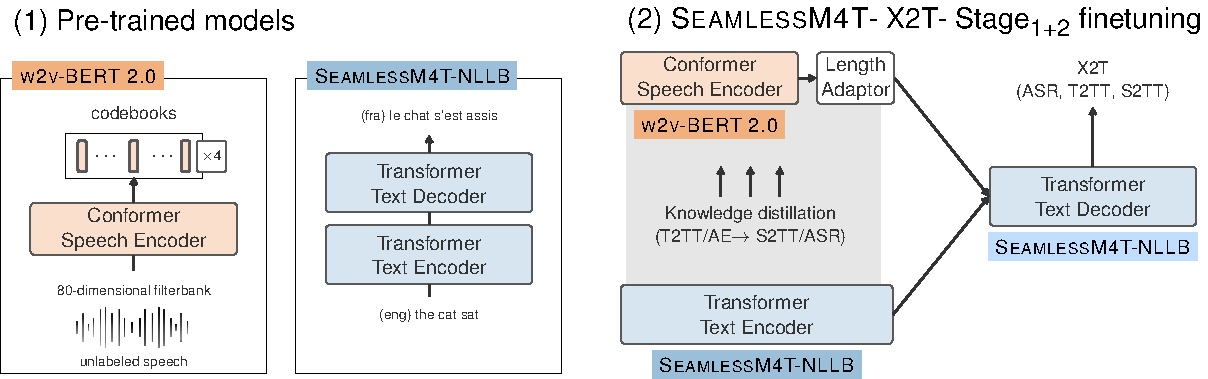
\includegraphics[width=\linewidth]{figures/modeling/modeling_x2t_flow.pdf}    \caption{\textbf{Overview of the \mfourt~\xt model.} (1) describes the main two building blocks: \wvbert and \nllbv. (2) describes the training of the \xt model. In $\text{Stage}_1$, the model is trained on \xeng directions and in $\text{Stage}_2$, \engx directions are added.}
    \label{fig:modeling:flow:x2t}
\end{figure}
The core of our multitask \unity framework is the \xt model, a 
multi-encoder
sequence-to-sequence models with a Conformer-based encoder~\citep{gulati2020conformer} for speech input and another for Transformer-based encoder~\citep{vaswani2017attention} for text input—both of which are joined 
with the same text decoder.
Our \xt model is trained on \st data pairing speech audio in a source language with text in a target language.

\subsubsection{Preparing \xt data}\label{sec:modeling:x2t:data}
\begin{figure}[tbh]
\centering

\includegraphics[width=\linewidth]{modeling/asr_s2t_data_counts_horizonal}
\caption{Statistics of \asr and \xeng~\st data used to train our \mfourt model. We show the data size in hours of speech (log-scale) between \asr, \st primary and mined. Languages are sorted in ascending resource-level.
For numerical statistics see \Cref{tbl:modeling:s2tdata}}
\label{fig:s2tdata}
\end{figure}
\paragraph{Processing human-labeled data}
When using human-labeled data, we removed special tokens such as \texttt{<silence>} and \texttt{<no-speech>} from the verbatim transcriptions. 
We additionally perform length filtering to remove examples exceeding a maximum text length of 100 sub-word tokens 
(based on the text tokenizer described below) 
and pairs with a skewed text-to-audio length ratio that exceeds 5 sub-words per second. 
Doing so improves the batching efficiency when training and eliminates pairs that are likely to be noisy or misaligned.

\paragraph{Pseudo-labeling}
As with any sequence-to-sequence task, \st performance is dependent on the availability of high-quality training data. However, the amount of human-labeled \st data is scarce in comparison to its \mt or \asr counterparts. To address this shortage of labeled data, we resort to pseudo-labeling~\citep{jia2019leveraging, Pino2020SelfTrainingFE} the \asr data with a multilingual \mt model. In this case, we used NLLB-200-3.3B and generated pseudo-labels with the recommended decoding options from \cite{nllb2022}. Hereafter, we refer to human-labeled and pseudo-labeled data as \textit{primary} data. %

\paragraph{Parallel data mining}
Even with pseudo-labeled \asr data, the amount of \st data is insignificant compared to the scale of \mt data.
Consider for instance the English-Italian direction, one of the highly resourced pairs in \mt with over 128M parallel sentences—only 2M pairs of English text paired with Italian audio are available for \st.
Parallel data mining (see how \mineddata was built in \Cref{sec:appendix:data}) is another strategy we draw upon to collect more training data. 
This kind of mining, however, 
tends to produce noisy alignments and requires some filtering.
We use the top 400 hours 
of \mineddata (see \Cref{sec:appendix:data}) in each of 33 \xeng directions and the top 200 hours in each of 29 \engx directions based on \sonar alignment scores.
This amounts to an additional 18.3K hours of speech audio. 
We show in \Cref{{sec:modeling:ablation:data}} that these select amounts of mined data lead to a good trade-off between performance boosts and computational costs of training.

\paragraph{Filtering}\label{sec:modeling:filtering}
We perform additional filtering on the combined pool of \textit{primary} and \textit{mined} data.
Following \cite{nllb2022}, we implemented a toxicity filter. This removes pairs that have \emph{toxicity imbalance}, (i.e., when the difference in the number of toxic items detected in the source and target is above a certain threshold). For \st data, transcriptions are used as a proxy for the speech input when counting toxic items. We set the imbalance threshold at 1. 
In addition, we also applied a length filter. We removed pairs in which the utterance is shorter than 0.1 seconds or longer than 50 seconds. We also removed pairs in which the text is longer than 250 sub-words (based on the tokenizer described below). Lastly, we removed pairs in which the text contains more than 20\% of emojis, more than 50\% of punctuations, or more than 50\% of spaces.


\Cref{fig:s2tdata} shows the distribution of filtered \xeng~\st data used to train \mfourt models. Based on the total amount of speech audio hours in each language, we assessed its resource level: \textit{high-resource} are languages with more than 1000 hours of supervision, \textit{mid-resource} are those between 500 and 1000 hours, and \textit{low-resource} are those with less than 500 hours.

\paragraph{Training a Text Tokenizer.}
The tokenizer used in NLLB-200~\citep{nllb2022} is trained with \textit{SentencePiece}~\citep{sentencepiece} using the BPE algorithm~\citep{gage1994new,sennrich-etal-2016-neural}. 
These multilingual tokenizers, with their underlying vocabularies, are trained by sampling data from each language. Due to artifacts of sampling and the much larger number of unique symbols in logo-graphic writing systems, the result of this is that many key Chinese characters are missing from the original NLLB-200 vocabulary. To address this issue, we force the inclusion of these characters even in cases where they may not appear in the sampled \textit{SentencePiece} training data.
In order to decide which characters to include, we looked at the MTSU list\footnote{\url{https://lingua.mtsu.edu/chinese-computing/statistics/index.html}} and similar character frequency lists obtained from mined data in order to select the top 5000 Simplified Chinese characters, Traditional Chinese characters, and Japanese kanji characters. We then forced their inclusion, as long as they appeared at least 15 times in our training data to guarantee that the model would be able to learn how to embed these tokens.

We re-trained a 256K-sized \textit{SentencePiece} vocabulary on NLLB data~\citep{nllb2022} for \mfourt. The resulting tokenizer improves the coverage of the MTSU top 5K Chinese characters from 54\% to 84\%.

\subsubsection{Training a Large-Scale Multilingual Text-to-Text Translation Model}\label{sec:modeling:x2t:nllb}
We follow the same data preparation and training pipelines from \cite{nllb2022} using \stopes~\citep{andrews-etal-2022-stopes}. Having a smaller language coverage (100 instead of NLLB's 200 languages) allowed us to significantly decrease the size of the model. Whereas the full NLLB-200 model with mixture-of-experts is made up of 54.5B parameters (a number which can later be decreased via distillation), we opted for one of the smaller architectures proposed in \cite{nllb2022}, the 1.3B dense model.
We limited the NLLB-200 training data to the \ntextlangs \mfourt languages to be supported as target text. 
We additionally included over 75M bitexts from open-source \mt datasets that were not included in \cite{nllb2022}. These concern 
Modern Standard Arabic (arb), Mandarin Chinese (cmn), French (fra), Russian (rus), and Spanish (spa).
\begin{table}[!t]
\centering
\small
\begin{tabular}{@{}lcc@{}}
\toprule
& \multicolumn{2}{c}{\bf \mt ($\uparrow$\chrf)} \\\cmidrule{2-3}
{\bf Model} & \makecell[c] {\xeng\\ {\it (n=95)}}	&   \makecell[c] {\engx \\ {\it (n=95)}}\\
\midrule
\cite{nllb2022} & &\\
~- 3.3B  &	60.6 &	\bf 49.6 \\
~- 1.3B  &	59.3 &	48.2 \\
~- 1.3B-distil.  &	59.5 &	48.8 \\
\midrule
\nllbv-1.3B	& \bf 60.7	& \bf 49.6 \\ 
\bottomrule
\end{tabular}
\caption{Average \flores devtest \chrf over the \ntextlangs supported languages.}\label{tbl:nllb-v2-chrf}
\end{table}

We compare in \Cref{tbl:nllb-v2-chrf} the performance of \nllbv to that of comparably-sized NLLB models on \flores, averaging over our \ntextlangs languages when translating from English (\engx) and into English (\xeng). The model outperforms both smaller models from NLLB-200 (1.3B and 1.3B-distil) and is on par with the larger 3.3B model.

\subsubsection{Multimodal \& multitask into target text}\label{sec:modeling:x2t:stage12} 
In \mfourt, we leveraged foundational models either pre-trained on unlabeled data (w2v-BERT 2.0 for speech encoder pre-training) or trained on supervised high-resource tasks (NLLB model for \mt) to improve the quality of transfer tasks (speech-to-text and speech-to-speech). To fuse these pre-trained components and enable meaning transfer through multiple multimodal tasks, we trained an end-to-end model with (a) a speech encoder (\wvbert) postfixed with a length adapter, (b) text encoder (NLLB encoder), and (c) a text decoder (NLLB decoder). 
For the length adaptor, we used a modified version of M-adaptor~\citep{zhao22g_interspeech}, where we replaced the 3 independent pooling modules for Q, K, and V with a shared pooling module to improve efficiency.

The model is fine-tuned to jointly optimize the following objective functions:
\begin{align}
    \mathcal L_{\text{\st}} & = - \sum_{t=1}^{|y|} \log p(y^\text{text}_t | y^\text{text}_{<t}, x^\text{speech}),\\
    \mathcal L_{\text{\mt}} & = - \sum_{t=1}^{|y|} \log p(y^\text{text}_t | y^\text{text}_{<t}, x^\text{text}),
\end{align}
where $x^\text{text}$ and $x^\text{speech}$ are the source text and speech in the source language ${<}\ell_s{>}$ and $y^\text{text}$ is the target text in the target language ${<}\ell_t{>}$.
We additionally optimize an auxiliary objective function in the form of token-level knowledge distillation ($\mathcal{L}_{\text{KD}}$), to further transfer knowledge from the strong MT model 
to the student speech translation task (\st).
\begin{align}
    \mathcal{L}_{\text{KD}} & = \sum_{t=1}^{|y|} D_\text{KL}
    \left[
    p(. |y^\text{text}_{<t}, x^\text{text})\, \| \,
    p(. |y^\text{text}_{<t}, x^\text{speech})
\right].
\end{align}
The final loss is a weighted sum of all three losses:
    $\mathcal L = \alpha \mathcal{L}_{\text{\st}} + \beta \mathcal{L}_{\text{\mt}}+ \gamma \mathcal{L}_{\text{KD}},$
where $\alpha, \beta, \gamma$ are scalar hyperparameters tuned on the development data.
When the task does not fit the design of data triplets, we
then replaced translation tasks with auto-encoding—for example, on \asr $y^\text{text}$ is replaced by $x^\text{text}$ 
in which case the teacher distribution is from auto-encoding ($p(. |x^\text{text}_{<t}, x^\text{text})$).

We trained our \xt model in two stages. $\text{Stage}_1$ targeted training on supervised English \asr and into English \st data. We find that this step is necessary not only for improving the quality of \xeng translations but also \engx translations. In fact, we hypothesized that allowing the model to focus on one target language while fine-tuning multilingual speech representations shields it from the interference that can propagate back from the target side. In $\text{Stage}_2$, we add supervised \engx~\st and non-English \asr data to the mix. 


\subsection{Speech-to-Speech Translation}\label{sec:modeling:s2st}
\begin{figure}[!htb]
    \centering
    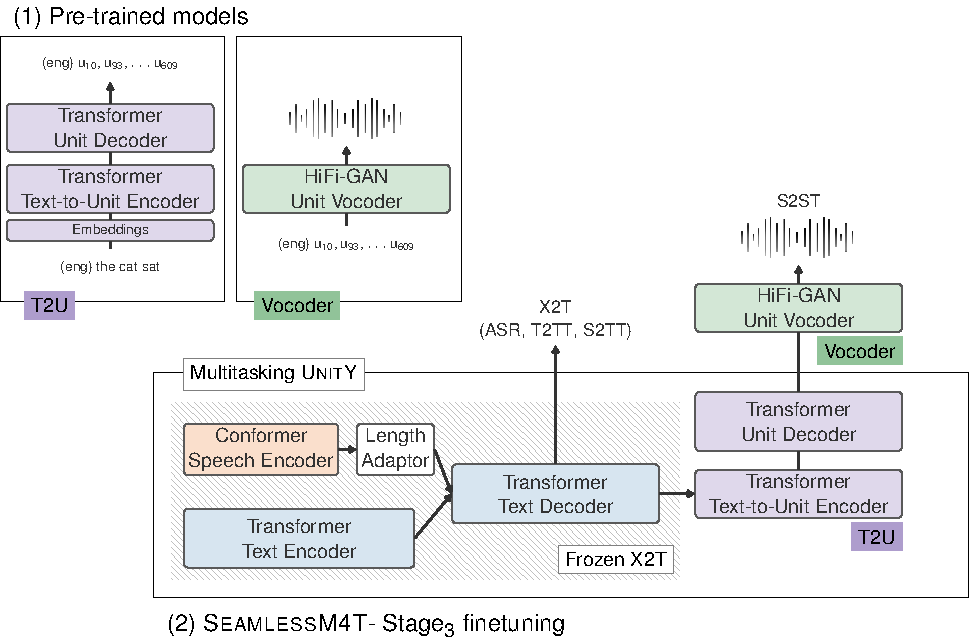
\includegraphics[width=\linewidth]{figures/modeling/modeling_s2st_flow.pdf}
\caption{
\textbf{Overview of the \mfourt multitask \unity model.} (1) describes the additional two building blocks on top of \xt: \tu encoder-decoder and unit vocoder. (2) describes the training of the \unity model. In $\text{Stage}_3$, the model is trained on \sst data.
}
\label{fig:modeling:flow:s2st}
\end{figure}
The key to our proposed speech-to-speech translation model is the use of self-supervised discrete acoustic units to represent target speech, thereby decomposing the S2ST problem into a speech-to-unit translation (S2UT) step and a unit-to-speech (U2S) conversion step.
For S2UT, the \mfourt model depicted in \Cref{fig:modeling:overview} uses \unity as a two-pass decoding framework which first generates text and
subsequently predicts discrete acoustic units.
Compared to the vanilla \unity model~\citep{unity}, 
(1) the core \st model initialized from scratch is replaced with an \xt model pre-trained to jointly optimize \mt, \st, and \asr,
(2) the shallow T2U model (referred to as T2U unit encoder and second-pass unit decoder in \cite{unity}) is replaced with a deeper Transformer-based encoder-decoder model with 6 transformer layers,
(3) the T2U model is also pre-trained on the T2U task rather than trained from scratch. 
The pre-training of \xt yields a stronger speech encoder and a higher quality first-pass text decoder,
while the scaling and pre-training of the T2U model allowed us to better handle multilingual unit generation without interference. 



\subsubsection{Preparing \sst data}\label{sec:modeling:s2st:data}
\paragraph{Discrete acoustic units}
Recent works have achieved SOTA translation performance by using self-supervised discrete acoustic units as targets for building direct speech translation models~\citep{tjandra2019speech,lee-etal-2022-direct,lee-etal-2022-textless,zhang-etal-2022-speechut,chen-etal-2023-speech}. 
We extracted features from the 35$^\text{th}$ layer of \xlsr-1B~\citep{babu2021xls} for continuous speech representations at a 50Hz frame rate.
The mapping from \xlsr continuous representation space to discrete categories is required to map target speech into a sequence of discrete tokens. 
We randomly selected and encoded 10K unlabeled audio samples from each language of the \ntslangs supported target languages.
We then applied a $k$-means algorithm on these representations to estimate $K$ cluster centroids~\citep{lakhotia-etal-2021-generative,polyak21_interspeech,lee-etal-2022-direct}. 
These centroids resemble a codebook that is used to map a sequence of \xlsr speech representations into a sequence of centroid indices or acoustic units.
Experiments with different numbers of centroids ($K\in\{1000, 2000, 5000, 10000\}$) show that $K{=}10000$ with features from the 35$^\text{th}$ layer of \xlsr-1B achieves the best speech re-synthesis \wer~\citep{polyak21_interspeech}.

\xlsr has a broader language coverage than existing HuBERT~\citep{hsu2021hubert} models, and we found it provided similar speech re-synthesis performance to HuBERT on overlapping languages. We also experimented with \wvbert, which showed inferior performance. This can be attributed to w2v-BERT training with contrastive and MLM objectives, encouraging the model to only learn about semantic tokens rather than acoustic ones.

\paragraph{Synthesizing multilingual units with HiFi-GAN}
Following \cite{gong2023multilingual}, we built the multilingual vocoder for speech synthesis from the learned units. The HiFi-GAN vocoder~\citep{kong2020hifi} is equipped with language embedding to model the language-specific acoustic information. Moreover, to mitigate cross-lingual interference, language identification is used as an auxiliary loss in multilingual training.
We used a combination of commissioned and publicly available datasets, including single-speaker and multi-speaker \tts datasets, to train the multilingual vocoder on \nvocoderlangs target languages capable of converting the discrete units predicted by our S2UT model into waveforms. 
Compared to monolingual vocoders, we increased the model capacity by doubling the embedding dimension for both 
the duration predictor 
and the speech-language identification (LID) classifier to reach 1280.
\begin{figure}[!t]
\centering

\includegraphics[width=\linewidth]{modeling/s2st_data_counts}
\caption{Statistics of \sst data used in $\text{Stage}_3$ of training \mfourt model. We show the data size in hours of speech between primary and mined. Languages are sorted in ascending resource-level.
For numerical statistics see \Cref{tbl:modeling:s2stdata}}
\label{fig:s2stdata}
\end{figure}
\paragraph{Pseudo-labeling with text-to-unit}
The insufficient amount of parallel speech-to-speech training data significantly limits the training of high-quality S2UT models. To overcome this data scarcity, it is common practice to use \tts models to convert text from speech-to-text datasets (see \Cref{sec:modeling:x2t:data}) into synthetic speech~\citep{jia:interspeech:2019,lee-etal-2022-direct}.
This synthetic speech is in turn converted into units using the previously described unit extraction pipeline. This two-step unit extraction process is a slow process and is harder to scale given the dependencies on \tts models. 
High-quality off-the-shelf \tts models are hard to come by for all languages, especially for low-resource ones. Training reliable monolingual or multilingual in-house \tts models is also not scalable given the challenges around gathering high-quality clean speech data.
To overcome these challenges, we circumvented the need for synthesizing speech and trained multilingual text-to-unit (T2U) models on all the \nvocoderlangs target speech languages. 
These models can directly convert the text into target discrete units and can be trained on \asr datasets that are readily available. 
The multilingual training benefits from cross-lingual transfer between high-resource and low-resource languages, thereby also improving the quality of the pseudo-labeled data. To remove outlier samples from our paired data, we filtered based on the number of seconds of audio generated per text token length ratio, discarding any pair with a ratio exceeding 0.5.


\paragraph{Parallel data mining: \mineddata}
We added up to 2,500 hours of mined speech-to-speech data from \mineddata per language direction depending on its availability (see \Cref{sec:appendix:data}) . We used the XLSR-based unit extraction pipeline for extracting discrete acoustic units for target speech from the mined data. An in-house ASR model is then deployed to generate text transcriptions for the first pass decoder based on the target speech.


\Cref{fig:s2stdata} shows the distribution of all \sst data used to train \mfourt models between the primary and mined data.

\subsubsection{T2U modeling}\label{sec:modeling:s2st:t2u}
The T2U model is a Transformer-based encoder-decoder model trained on aligned text units from ASR data.
We trained T2U models for two purposes: (1) performing pseudo-labeling (\Cref{sec:modeling:s2st:data}) and (2) initializing the T2U component in \unity. 
For (1), 
we trained a model with 12 encoder and 12 decoder layers.
For (2), we trained a smaller T2U model with 6 encoder and 6 decoder layers.
Initial experiments showed that, although the smaller T2U model is of a lower quality than the larger one, fine-tuning the smaller T2U in \unity with labels from the larger one (i.e., distilling knowledge from the stronger T2U) can bridge the gap while being parameter-efficient.


\subsubsection{$\text{Stage}_3$ Finetuning for \sst}\label{sec:modeling:s2st:stage3}
In the last stage of fine-tuning, we initialized the multitask \unity model (see \cref{fig:modeling:overview}) with (1) the pre-trained \xt model and (2) the pre-trained T2U model and fine-tuned on a combination of \xeng and \engx~\sst translation data totaling 121K hours (see breakdown in \cref{fig:s2stdata}).
We froze the model weights corresponding to the \xt model and only fine-tuned the T2U component. This is to ensure that the performance of the model on tasks from the previous stages of fine-tuning remains unchanged. 

\subsection{The \mfourt Models}\label{sec:modeling:main}
With all the components laid out in the previous sections, we trained the \mfourtlg model in the outlined three stages. 
\mfourtlg has 2.3B parameters and is fine-tuned on
\mt for \ntextlangs languages paired with English, on \asr for \nasrlangs languages, 
on \st for 89 languages paired with English, and on \sst for 95 directions into English and \ntslangs target languages out of English. 
The amount of supervised data per direction is detailed in \cref{tbl:modeling:s2stdata,tbl:modeling:s2tdata}. This means that, for some source languages, our models are evaluated zero-shot to reach the coverage described in \cref{tbl:coverage} of \nsslangs-eng.

To provide a reasonably sized model, we followed the same recipe to train \mfourtmd. This model has 57\% fewer parameters than \mfourtlg and is intended to be an accessible test bed to either fine-tune, improve on, or engage in analysis with. \mfourtmd has the same coverage as \mfourtlg but builds on smaller and more parameter-efficient components (see \Cref{fig:modeling:overview}). 
We pre-trained a smaller \wvbert with 300M parameters and used the distilled model from \cite{nllb2022} (\nllbtinydistil) to initialize the \mt{} modules of the multitask \unity. See a comparison between \mfourtlg and \mfourtmd in \Cref{tbl:modeling:collection}. 
\begin{table}[!ht]
    \centering
    \small
    \begin{tabular}{ccccc}
    \toprule
          & {\bf $\text{\wvbert}^*$} & {\bf \mt} & {\bf T2U}  & {\bf Total} \\
    \midrule
\mfourtlg & 669M & 1370M & 287M & 2326M  \\
\mfourtmd & 366M & 615M & 170M & 1151M \\
    \bottomrule
    \end{tabular}
    \caption{\#parameters of the building components used  in \mfourt models.\\
    *: includes the parameters of the length adaptor .\\
    }
    \label{tbl:modeling:collection}
\end{table}

We evaluated our models on all four supervised tasks (\mt, \asr, \st, and \sst) as well as the zero-shot task of text-to-speech translation (\ttst, also referred to as cross-lingual text to speech synthesis~\citep{Zhang2023SpeakFL}). 
To generate text hypotheses, we decoded with beam-search (width${=}5$).
We scored with \chrf for \mt
and SacreBLEU for \st (default 13a tokenizer and character-level tokenizer for Mandarin Chinese (cmn), Japanese (jpn), Thai (tha), Lao (lao), and Burmese (mya); see signatures in \Cref{tbl:eval:metrics}).
For \asr, we scored with \wer on normalized transcriptions and references following \cite{whisper}.

During \sst and \ttst inference, we performed two-pass beam-search decoding— 
the best hypothesis out of the first-pass decoding is embedded with the text decoder and is sent to T2U to search for the best unit sequence hypothesis. We use a beam-width of 5 for both searches. We evaluated \sst and \ttst accuracy with \asrbleu~\citep{lee-etal-2022-direct} with \whisperlarge as the underlying \asr model for \engx directions and with \whispermedium for \xeng directions. We set the decoding temperature of Whisper at zero and used greedy decoding to ensure a deterministic behavior of the ASR model.
The transcribed hypotheses, as well as the references, are normalized following \cite{whisper} before computing \bleu scores in the same manner we did for \st. 


\subsubsection{Comparison to cascaded approaches.}
On the set of languages supported by both \mfourt and Whisper, we compare in \Cref{tbl:modeling:cascaded:x2t} the performance of our direct \st model to that of cascaded models, namely combinations of Whisper \asr models and NLLB \mt models.
%
\mfourtlg surpasses the cascaded models with less than 3B of parameters  in \xeng directions by 2 \bleu points and in \engx directions by 0.5 \bleu points. We also add to the comparison in \Cref{tbl:modeling:cascaded:x2t} cascaded models with the large \nllbmedium~\mt model. These models exceed 4B parameters and only outperform \mfourtlg in \engx directions. \mfourtlg improves on \whisperlarge+\nllbmedium by 1.3 \bleu points on average in \xeng directions.

\Cref{tbl:modeling:cascaded:s2st} compares \sst between \mfourtlg and cascaded models. For \sst, we look at two options for cascading: (1) 3-stage with \asr, \mt, and \tts and (2) 2-stage with \st and \tts. 
Our \mfourtlg outperforms 2-stage cascaded models on \fleurs~\xeng directions by 9 \asrbleu points. It also outperforms stronger 3-stage cascaded models (\whisperlarge + \nllbmedium  + \yourtts) by 2.6 \asrbleu points. On \cvss, \mfourtlg outperforms the 2-stage cascaded model (\whisperlarge + \yourtts) by a large margin of 14 \asrbleu points. 
On \fleurs~\engx directions, \mfourtlg has an average \asrbleu of 21.5 on 32 \xeng directions excluding target languages where \whisperlarge (the \asr model used for \asrbleu) has a \wer higher than 100. Comparably, the medium-size model (\mfourtmd) scores an average \asrbleu of 15.4 on \sst~\engx directions.

\begin{table}[!ht]
    \centering
    \small
    \begin{tabular}{@{}lcccc@{}}
        \toprule
         &  &  & \multicolumn{2}{c}{\makecell[c]{\bf \st ($\uparrow$\bleu)}} \\
        \cmidrule{4-5}
         {\bf Model} & {\bf  type} &  { \bf size}  & \makecell[c]{\xeng \\{\it (n=81)}} & \makecell[c]{\engx\\{\it (n=88)}} \\
         \midrule
        \whispermedium (\asr)\phantom{a} + \nllbsmall & \multirow{4}{*}{cascaded} &  2B &  19.7 & 20.5 \\
        \whispermedium (\asr)\phantom{a}  + \nllbmedium &  &  4B &  20.4 & 21.8 \\
        \whisperlarge (\asr)+ \nllbsmall &  & 2.8B & 22.0 & 21.0 \\
        \whisperlarge (\asr)+ \nllbmedium &  & 4.8B & 22.7 & \bf 22.2  \\
        \midrule
        \whisperlarge & \multirow{2}{*}{direct} & 1.5B & 17.9 & - \\
        AudioPaLM-2-8B-AST &  & 8B & 19.7 & - \\
\midrule
        \mfourtmd & \multirow{2}{*}{direct} & 1B & 20.9 & 19.2 \\
        \mfourtlg &  & 2B & \bf 24.0 & 21.5 \\
        \bottomrule
    \end{tabular}
\caption{Comparison against cascaded \asr+\mt models on  \fleurs~\st.}\label{tbl:modeling:cascaded:x2t}
\end{table}

\begin{table}[ht]
    \small
    \centering
    \begin{tabular}{@{}lcccc@{}}
        \toprule
         &  &  & \multicolumn{2}{c}{\makecell[c]{\bf S2ST~\xeng \\\bf($\uparrow$\asr-BLEU)}} \\
        \cmidrule{4-5}
        {\bf Model} & {\bf type} & {\bf  size } & \makecell[c]{\fleurs \\{\it (n=81)}} & \makecell[c]{\cvss \\{\it (n=21)}}\\
        \midrule
       \multicolumn{4}{l}{\yourtts~\citep{casanova2022yourtts}}\\
       \phantom{abcd}+\whisperlarge (\st)  & \makecell[c]{2-stage\\cascaded} & 1.6B & 17.3 & 22.6 \\
       \midrule
       \phantom{abcd}+\whispermedium (\asr) \phantom{a}+ \nllbsmall &  \multirow{4}{*}{\makecell[c]{3-stage\\cascaded}}  &  2.1B &  19.9 & \\  
        \phantom{abcd}+\whispermedium (\asr)\phantom{a} + \nllbmedium &  &  4.1B &  20.6 & \\
        \phantom{abcd}+\whisperlarge (\asr)+ \nllbsmall &  & 2.9B & 22.1 & \\
        \phantom{abcd}+\whisperlarge (\asr)+ \nllbmedium &  & 4.9B & 23.2 &  \\
        \midrule
        \mfourtmd & unified & \sizemd & 20.4  & 28.1 \\
        \mfourtlg & unified & \sizelg & \bf 25.8  & \bf 36.5\\
        \bottomrule
    \end{tabular}
    \caption{Comparison against 2/3-stage cascaded models on \fleurs and \cvss~\sst~\xeng.}\label{tbl:modeling:cascaded:s2st}
\end{table}

\subsubsection{Multitasking \xt results.} \label{subsec:multitaskingxtresults}
\begin{table}[!t]
\small
    \centering
    \begin{tabular}{@{}lHccccc@{}}
        \toprule
         &  &  & \multicolumn{4}{c}{ \bf \st ($\uparrow$\bleu) }\\
        \cmidrule{4-7}
        
        {\bf Model}  & {\bf type} & \multirow{2}{*}{\makecell[c]{\bf size}} & \makecell[c]{\fleurs\\\xeng \\{\it (n=81)}} & \makecell[c]{\fleurs\\\engx \\{\it (n=88)}} & \makecell[c]{\covost\\\xeng \\{\it (n=21)}} & \makecell[c]{\covost\\\engx\\ {\it (n=15)}} \\
        \midrule
        \makecell[l]{\xlsrstot} & direct & 2.6B &  & x & 22.1 & 27.8 \\
        \makecell[l]{\whisperlarge} & direct & 1.5B & 17.9 & x & 29.1 & x \\
        \makecell[l]{\audiopalmast}  & direct & 8.0B & 19.7 & x & \bf 37.8 & x \\
        \midrule
        \mfourtmd & direct & \sizemd & 20.9 & 19.2 & 29.8 &  26.6 \\
        \mfourtlg & direct & \sizelg & \bf 24.0 & \bf 21.5 & 34.1 & \bf 30.6  \\  
        \bottomrule
    \end{tabular}\\[10pt]
     \begin{tabular}{@{}lHccccc@{}}
        \toprule
         &  &  & \multicolumn{2}{c}{\bf \asr ($\downarrow$WER) } & \multicolumn{2}{c}{\bf \mt ($\uparrow$\chrf)}\\
        \cmidrule(r){4-5}
        \cmidrule(l){6-7}
        {\bf Model}  & Model type & \multirow{2}{*}{\makecell[c]{\bf size}} & \makecell[c]{\fleurs \\ {\it (n=77)}} & \makecell[c]{ \fleurs-54\\ {\it (n=54)} }  & \makecell[c]{\flores\\\xeng\\{\it (n=\ntextlangs)}} & \makecell[c]{\flores\\\engx\\{\it (n=\ntextlangs)}} \\
        \midrule
        \nllbmedium & direct & 3.3B & x & x & 60.7 & 49.6 \\
        \midrule
        \makecell[l]{\whisperlarge} & direct & 1.5B & 41.7 & 43.7 & x & x \\
        \makecell[l]{MMS-L61-noLM-LSAH} & direct & 1.0B & x & 31.0 & x & x \\
        \makecell[l]{MMS-L1107-CCLM-LSAH} & direct & 1.0B$^*$ & x & \bf 18.7 & x & x \\
        \midrule
        \mfourtmd & direct & \sizemd & \bf 21.9 & 22.0 & 55.4  & 48.4 \\
        \mfourtlg & direct & \sizelg & 23.1 & 23.7 &  \bf 60.8 & \bf 50.9 \\
        \bottomrule
    \end{tabular}
    \caption{\textbf{Multitasking \xt results.} Performance of \mfourtlg on \xt tasks (\st, \asr and \mt) compared to SOTA direct translation models. 
    For \fleurs~\st~\xeng, we report the average \bleu scores over languages Whisper supports.
    For \fleurs~\asr, we report the average normalized \wer over languages supported by both \mfourt and Whisper.
    For MT, we average \chrf~scores over the supported written languages in \mfourt. 
    *: MMS is CTC-based, and this version decodes with an n-gram language model for each language.
    Note that for all external models included in this comparison, we lifted the results reported in their respective papers and matched their evaluation and scoring pipeline for a fair comparison.\protect\footnotemark
    }
    \label{tbl:modeling:main:x2t}
\end{table}
\footnotetext{
Scoring \whisperlarge, using \url{https://github.com/openai/whisper} with the recommended decoding options, results in \bleu scores lower by 0.3 \bleu points on average than what is reported in~\cite{whisper}.
}
\begin{table}[!htb]
    \centering
    \small
    \begin{tabular}{@{}lcccc@{}}
        \toprule
         & \multicolumn{4}{c}{\bf \fleurs~\st~\xeng ($\uparrow$\bleu)}  \\\cmidrule{2-5}
          {\bf Model} & \makecell[c]{High\\ {\it (n=15)}} &\makecell[c]{ Medium\\ {\it (n=25)}} & \makecell[c]{Low \\ {\it (n=34)}}& \makecell[c]{Low$^\dagger$ \\ {\it (n=23)}} \\
        \midrule

        \whisperlarge & 24.2 & 19.4 & 16.1 & 18.1 \\
        \audiopalmast & \bf 27.9 & 20.9 & 18.0 & 22.0 \\
        \midrule
        \mfourtmd & 23.9 & 21.8 & 22.2 & 23.5 \\
        \mfourtlg & 26.9 & \bf 25.2 & \bf 25.4 & \bf 27 \\        
        \bottomrule
    \end{tabular}
    \caption{\textbf{\fleurs~\st~\xeng by resource-level.} In each resource-level (high, medium and low), we average over languages that are covered by all 3 models. In low$^\dagger$, we exclude low-resource languages that are evaluated as zero-shot by \audiopalmast.}
    \label{tbl:modeling:s2t:res}
\end{table}
\begin{table}[!t]
\small
    \centering
    \begin{tabular}{@{}lHccccccc@{}}
        \toprule
         {\bf Model} & Model type 
         & \multirow{2}{*}{\makecell[c]{\bf size}} 
         & \multicolumn{3}{c}{\makecell[c]{\fleurs~\xeng {\it (n=81)}}}
         & \multicolumn{3}{c}{\makecell[c]{\fleurs~\engx {\it (n=88)}}} \\  
         \cmidrule(l){4-6}  \cmidrule(r){7-9}
        &  &  
        & \scriptsize$\uparrow$\bleu 
        &\scriptsize$\uparrow$\spbleu  
        &\scriptsize$\uparrow$\blaser
        &\scriptsize$\uparrow$\bleu 
        & \scriptsize$\uparrow$\spbleu  
        & \scriptsize$\uparrow$\blaser \\
        \midrule
        \makecell[l]{\whisperlarge} & direct 
                & 1.5B & 17.9 & 19.9 & 3.29  & x & x & x \\
        \midrule
        \mfourtmd & direct & \sizemd 
        & 20.9 & 23.1 & 3.56 
        & 19.2 & 26.0 & 3.68 \\
        \mfourtlg & direct & \sizelg 
        & \bf 24.0 &\bf 26.4 & \bf 3.66 
        & \bf 21.5 & \bf 28.9 & \bf 3.71\\
        \bottomrule
    \end{tabular}
    \caption{\textbf{\st results with \spbleu and \blaser} we report here the performance of \whisperlarge and \mfourtlg measured with \spbleu \& \blaser. Note that unlike \bleu scores copied from \cite{whisper}, the \spbleu and \blaser scores are based on our evaluation using \url{https://github.com/openai/whisper} with the recommended decoding options.
    }
    \label{tbl:modeling:spbleu}
\end{table}
\begin{table}[!t]
\small
    \centering
    \begin{tabular}{@{}lHHccccccc@{}}
        \toprule
         &  &  
         & \multicolumn{4}{c}{\bf \sst ($\uparrow$\asrbleu)}
        & \multicolumn{3}{c}{\bf \sst ($\uparrow$\blaser)}\\
        \cmidrule(l{2pt}){4-7} \cmidrule(r){8-10}
         {\bf Model} & Model type 
         & \multirow{2}{*}{\makecell[c]{\bf size}} 
         & \makecell[c]{\fleurs\\\xeng \\ {\it (n=101)}} 
          & \makecell[c]{\fleurs\\\xeng \\ {\it (n=82)}} 
         & \makecell[c]{\fleurs\\\engx\\ {\it (n=35)}}
         & \makecell[c]{\fleurs\\\engx\\ {\it (n=32)}}
         & \makecell[c]{\fleurs\\\xeng \\ {\it (n=82)}} 
         & \makecell[c]{\fleurs\\\engx\\ {\it (n=35)}}
         & \makecell[c]{\fleurs\\\engx\\ {\it (n=32)}}  \\
        \midrule
        \mfourtmd & & \sizemd  & 17.9 & 20.8 & 14.3 & 15.4 
        & 3.62 & 3.63 & 3.63
        \\ 
        \mfourtlg & & \sizelg & 22.7 & 26.3 & 19.8 & 21.5 
        & 3.85 & 3.94 & 3.95
        \\
        \bottomrule
    \end{tabular}
    \caption{\textbf{\sst results with \asrbleu and \blaser} we report here the performance of \mfourtlg and \mfourtmd measured with \asrbleu \& \blaser.
    }
    \label{tbl:modeling:sst:blaser}
\end{table}

We report in \Cref{tbl:modeling:main:x2t} results on the \fleurs benchmark for the tasks of \asr and \st (\xeng and \engx), and the related \flores benchmark for \mt (\xeng and \engx).
We also report results on the evaluation test set of \covost (\xeng and \engx)
The \mfourt model outperforms the previous direct SOTA model (AudioPaLM-2 8B AST~\citep{Rubenstein2023AudioPaLMAL}) by 4.2 \bleu points in \st \xeng directions (i.e., an improvement of 20\%).
In \covost~\engx, \mfourtlg improves upon the previous SOTA (\xlsr) by 2.8 \bleu points. However, in \xeng, it lags behind AudioPaLM by 3.7 \bleu points. 
For \asr, \mfourt outperforms Whisper~\citep{whisper} on the overlapping 77 supported languages with a \wer reduction of 45\%. 
We additionally compared against MMS~\citep{mms} on \fleurs-54, a subset of \fleurs languages that both MMS and Whisper support. \mfourtlg outperforms the MMS variants evaluated with CTC by more than 6\% WER, but it is surpassed by the variants that leverage
monolingual n-gram language models (5\% WER better). 

In the \mt support task, our \mfourt model matches the performance of NLLB-3.3B~\citep{nllb2022} in \xeng directions and improves on \engx directions by 1 \chrf point.
To further understand where the improvements in 
\fleurs~\st~\xeng directions are coming from, we bucket languages by resource-level (see the exact list of languages in \Cref{tbl:modeling:s2tdata}) and report average \bleu scores per resource-level in \Cref{tbl:modeling:s2t:res}. The results show that \mfourtlg strongly improves the quality of translating from low-resourced languages with an improvement of +7.4 \bleu (i.e., 40\% improvement over AudioPaLM-2-8B-AST). We also average in column low$^\dagger$ over low-resource directions that are supervised in AudioPaLM-2-8B-AST—the gain of +5 \bleu in that subset of directions suggests that this improvement goes beyond sheer supervision, but instead should be attributed to the quality of supervised data and the training recipes.


\subsubsection{Zero-shot Text-to-Speech Translation}\label{sec:modeling:t2st}
We evaluate \fleurs~\st on the reverse task of \ttst. We report in \Cref{tbl:modeling:t2st}
the average \asrbleu scores on 87 \xeng directions (the overlap between \fleurs and the languages supported by \mfourt text encoders). We also report the average \asrbleu on 32 \engx directions (excluding Bengali, Telugu and Northern Uzbek where \whisperlarge~\asr~\wer is above 100).
The \xeng average \asrbleu is higher than the \asrbleu of \sst~\xeng (34.9 vs. 24.6) where the \engx average is similar to that of \sst (22.5 vs. 21.5). This result demonstrates that (1) the quality of \mfourt on zero-shot \ttst is on-par with the supervised tasks and (2) that non-English speech source is the most challenging input to translate with our model.

\begin{table}[!tbh]
    \centering
    \small
    \begin{tabular}{@{}lccc@{}}
        \toprule
         & \multicolumn{2}{c}{\bf \fleurs~\ttst ($\uparrow$\asrbleu)}  \\
        \cmidrule(lr){2-4}
        {\bf Model} 
        &\makecell[c]{\xeng\\ {\it (n=88)}} 
        &\makecell[c]{\engx\\ {\it (n=35)}} 
        &\makecell[c]{\engx\\ {\it (n=32)}} \\
        \midrule
        \mfourtlg &  34.9 & 20.7 & 22.5  \\
        \bottomrule
    \end{tabular}
    \caption{\textbf{zero-shot \fleurs~\ttst} we report the average \asrbleu of \mfourtlg on \fleurs~\ttst.
    %
    }
    \label{tbl:modeling:t2st}
\end{table}

\subsubsection{Evaluation with \spbleu and \blaser.}
To avoid expanding the set of special case languages evaluated with character-level tokenization, we evaluated with \spbleu using the \flores-200 sentence piece tokenizer. \Cref{tbl:modeling:spbleu} reports \spbleu scores on \fleurs~\st~\xeng and \engx. 
We also report in the same table the average \blaser scores (for more on \blaser see \Cref{sec:eval:blaser}).
Since \blaser is modality-agnostic, we can also score the task of \sst with \blaser. 
\Cref{tbl:modeling:sst:blaser} provides the average \blaser scores of \mfourtlg and \mfourtmd on \sst~\xeng and \engx directions. Since \blaser supports 83 languages (including English), we average over 82 \xeng directions. For \engx, we show averages of 35 languages, then averages excluding 3 languages with a WER exceeding 100\%. Since \blaser supports all 35 target languages the scores are more reliable and less affected by the noisiness of the ASR model underlying \asrbleu (a difference of -1.7\asrbleu points with the addition of 3 directions).
The full results and metrics per evaluation direction can be found at \url{https://github.com/facebookresearch/seamless_communication}.
%

\subsubsection{Evaluation of \xy directions with \spbleu.}
Since \mfourt models support multiple languages on both the source and target sides, we can evaluate non-English centric directions (labeled \xy) in a zero-shot manner. 
\begin{figure}[!htb]
\centering
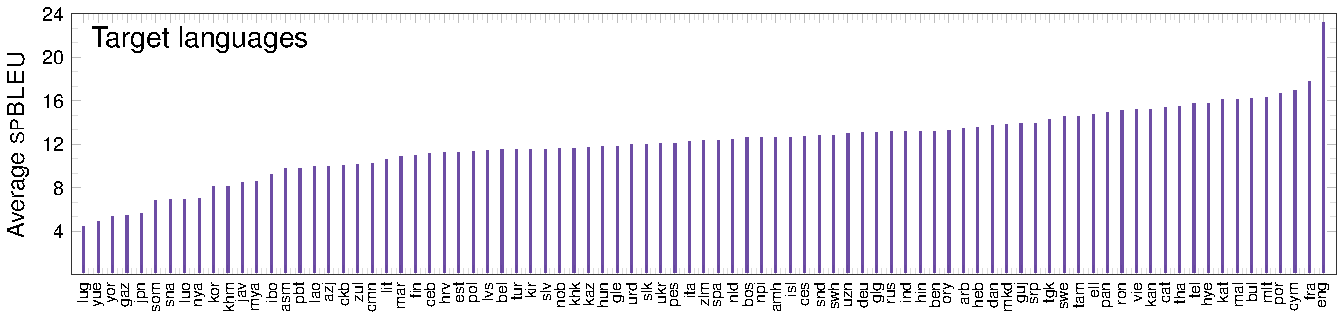
\includegraphics[width=\linewidth]{figures/modeling/fleurs_xx_results.pdf}
\caption{\textbf{\st~\fleurs~\xy results}. We evaluate \xy directions from \fleurs and average \spbleu scores. 
For a given target text language, we average scores over 100 source languages.
}\label{fig:modeling:x2t:xxresults}
\end{figure}
\FloatBarrier
\subsection{Analysis and Ablations}
\subsubsection{Unsupervised speech pre-training}
We explored various techniques to enhance the quality of our encoders’ representations, including 
algorithm-wise improvements and pre-training data scaling.

\begin{table}[t]
    \centering
    \small
    \begin{tabular}{@{}clHc@{}}
        \toprule
        \multirow{1}{*}{\bf ID} & \multirow{1}{*}{\bf Configuration} & &\multicolumn{1}{c}{\makecell[c]{\bf \fleurs~\xeng\\\bf($\uparrow$\bleu)}}\\
        \midrule
        A & w2v-BERT baseline with updated XLS-R data (400K hrs, 143 langs) & 16.1 & 12.4 \\
        B & A + product quantization with 2 GVQ codebooks & 16.3 & 12.5 \\
        C & B + increased open training data from 400K hours to 1M hours & 16.8 & 12.7 \\
        D & C + 2 RPQ codebooks for masked prediction objective & 17.0 & \bf 12.8 \\
        \bottomrule
    \end{tabular}
    \caption{Ablation on w2v-BERT variants and training data scaling.}\label{tbl:w2vbert}
\end{table}

\paragraph{Experimental setup}
In our ablation, we aimed to evaluate the w2v-BERT variants by their performance on the downstream \st task. All pre-trained w2v-BERT speech encoders are composed of 24 Conformer layers~\citep{gulati2020conformer} 
with approximately 600M of parameters. 
Each speech encoder was used to initialize an \st model.
The text decoder was initialized with the decoder from \nllbsmall, a large multilingual machine translation model covering 200 languages \citep{nllb2022} with 1.3B parameters.  
We fine-tuned the \st models on the task of speech translation into English (\xeng~\st) 
on
67 languages.
We fine-tuned all the speech encoder parameters and only fine-tuned LayerNorms and Self-attention in the text decoder (LNA-D~\citep{li-etal-2021-multilingual}). 
Our learning rate increased up to 3e-4 through 4000 warm-up updates and subsequently followed the inverse square root learning rate schedule. We trained on 32 GPUs with a batch size of 960K frames in each for 100K updates.
We report \bleu scores (SacreBLEU\footnote{see \Cref{tbl:eval:metrics}} \citep{post-2018-call}) evaluated on the test set of all 101 \xeng directions from \fleurs~\citep{fleurs2022arxiv}. 
Given the coverage of our training data, this means that 34 of the directions were evaluated as zero-shot.

\paragraph{Results}
We summarize our ablation results in~\Cref{tbl:w2vbert}. 
We see that product quantization with 2 GVQ codebooks outperforms normal quantization with a single GVQ codebook (A vs. B). Scaling training data leads to performance gains (B vs. C). Adding additional masked prediction learning objectives with 2 RPQ codebooks helps improve performance (C vs. D).

\begin{table}[!hb]
\centering
\footnotesize
\begin{tabular}{@{}cccccccccc@{}}
    \toprule
    \multirow{2}{*}{\makecell{\bf Language\\(code)}}  & 
   \bf \multirow{2}{*}{ASR} &
   \multicolumn{4}{c}{\bf \st} &
   \multicolumn{4}{c}{\bf \sst} \\
   \cmidrule(lr){3-6}
   \cmidrule(lr){7-10}
   & &
    \multicolumn{2}{c}{\xeng}&
    \multicolumn{2}{c}{\engx}&
    \multicolumn{2}{c}{\xeng}&
    \multicolumn{2}{c}{\engx} \\
     \cmidrule(l){2-2}
     \cmidrule(lr){3-4}
     \cmidrule(lr){5-6}
     \cmidrule(lr){7-8}
     \cmidrule(lr){9-10}
     & Primary & Primary & Mined & Primary & Mined & Primary & Mined & Primary & Mined \\
    
    \midrule
    arb & 934 
        & 942 & 600 
        & 1,959 & 600 
        & 899  & 736 
        & 895 & 681 \\
    ben & 338 
        & 320 & 600 
        & 1,987 & 499 
        & 292 & 246 
        & 652 & 221 \\
    eng & 3,845 & - & - &-  & - & - & - & - & - \\
    hin & 148 
        & 143 & 600 
        & 2,066 & 600 
        & 138 & 466 
        & 656 & 430 \\
    ind & 250 
        & 254 & 600 
        & 1,818 & 596 
        & 248 & 443 
        & 684 & 375 \\
    ita & 591 
    & 910 & 600 
    & 2,279 & 600 
    & 930 & 716 
    & 1,020 & 636 \\
    jpn & 381 
        & 15,141 & 600 
        & 1,798 & 259 
        & 624 & 993 
        & 681 & 779 \\
    por & 269 
        & 246 & 600 
        & 2,250 & 600 
        & 355 & 606 
        & 983 & 508 \\
    rus & 264 
        & 144 & 600 
        & 2,161 & 600 
        & 290 & 1,093 
        & 959 & 1,075 \\
    spa & 1,515 
        & 1,285 & - 
        & 2,505 & 574 
        & 1,694 & 2,335 
        & 1,035 & 2,209 \\
    swh & 361 
        & 50 & 600 
        & 1,930 & 596 
        & 342 & 411 
        & 682 & 392 \\
    tha & 190 
        & 59 & 600 
        & 1,941 & 101 
        & 184 & 462 
        & 641 & 408 \\
    tur & 169 
        & 100 & 600 
        & 2,135 & 600 
        & 156 & 375 
        & 998 & 411 \\
    urd & 185 
        & 145 & 600 
        & 1,844 & 507 
        & 179 & 555 
        & 682 & 502 \\
    vie & 194 
        & 151 & 600 
        & 2,396 & 600 
        & 176 & 666 
        & 954 & 684 \\
    \midrule
    \bf Total & 9,633  & 19,890 & 7,800 & 29,068 & 2,701 & 6,508 & 10,103 & 11,523 & 9,312 \\
    \bottomrule
\end{tabular}
\caption{Hours of data in the ablation dataset for the tasks of \asr, \st and \sst, split between \engx and \xeng when relevant. For each task, we report hours of training data between primary and mined. By default, \st mined data is capped at 400 hours in \xeng and at 200 hours in \engx.
}\label{tbl:s2t-ablation-dataset}
\end{table}
 
\subsubsection{Multimodal \& multitasking \xt}\label{sec:modeling:ablation:multitask}
\paragraph{Ablation dataset}
To iterate on different multitasking recipes, we constructed a smaller multilingual speech translation benchmark with 14 languages paired with English. 
The supervised \st data comes from two sources: primary (open-source or licensed) and mined, whereas the \asr data is either from open-sourced or licensed datasets.
The \mt data we used in our multitasking fine-tuning is limited to bitexts produced in the pseudo-labeling process, i.e., translated transcriptions in the \asr datasets (see \Cref{sec:modeling:x2t:data}).  
For a breakdown of the ablation dataset, see \Cref{tbl:s2t-ablation-dataset}.




\paragraph{Experimental setup}
We fine-tuned multilingual translation models on our ablation dataset with different mixes of tasks.
As a baseline, we only trained on primary \st data (\engx + \xeng), optimizing L1: $\mathcal L_\text{\st}$ exclusively.
With the data fixed, we experimented with two other objectives to optimize: (L2) with joint optimization of \mt and \st ($\mathcal L_\text{\st}+\mathcal L_\text{\mt}$) and (L3) with the additional knowledge distillation objective with \mt as the teacher and \st as the student.
We then added more data, namely \asr data and mined data respectively, and compared the performance of models trained with different objectives in the three data setups.

We initialized \xt models with our \wvbert speech encoder and  \nllbv \mt model. We fine-tuned all parameters in the speech encoder and text encoder, while only fine-tuning LayerNorms and Self-attentions in the text encoder (LNA~\citep{li2020multilingual}). We trained all models for 100K updates (corresponding to 5-7 epochs). To regularize our models, we applied LayerDrop ($p{=}0.1$) to the speech encoder with masking ($p{=}0.1$). For the text encoder-decoder, we applied regular dropouts ($p=0.1$). We evaluated the last checkpoint on development data and evaluated \bleu scores on \fleurs dev for translation tasks (including \mt) and Whisper-style normalized \wer for \asr.
\paragraph{Results}
Within each data setup (D1, D2 or D3), we see in \Cref{tbl:modeling:ablation:multitask} that adding \mt to the multitasking loss, as expected, helps the performance on \mt (+1.8 \bleu on average D1,2,3). Without adding this loss, fine-tuning exclusively on \st leads to catastrophic forgetting of the pre-training \mt task (comparing L1 to L2). However, the accuracy of \st is seldom affected by this joint training with \mt. Knowledge distillation is proving to be a necessary ingredient to leverage joint fine-tuning with \mt. After adding knowledge distillation (L1 to L3), \st's performance improves by 0.6 \bleu points on average (D1,2,3).

If we compare the three different data setups, adding \asr data is crucial to supporting the \asr task as evaluating it as zero-shot leads to $3\times$ higher error rates. Joint fine-tuning with \mt and the auxiliary knowledge distillation loss has no negative effect on \asr given that for \asr data, the teacher task is auto-encoding (see \Cref{sec:modeling:x2t:stage12}). Adding mined \st data for which the source text is not available for \mt to teach \st, still helps \st in the M3 task mix.
We note, however, that the accuracy of \mt drops as we add more speech-text only data (\asr and mined \st) without the aligned text-text data.

\begin{table}[tb]
    \centering
    \footnotesize
    \begin{tabular}{@{}lccccccccc@{}}
        \toprule
        Data & \multicolumn{3}{c}{\bf D1: \st data} & 
        \multicolumn{3}{c}{\bf D2: D1+\asr data} & 
        \multicolumn{3}{c}{\bf D3: D2+Mined data}  \\
        \cmidrule(r){2-4}
        \cmidrule(lr){5-7}
        \cmidrule(l){8-10}
        Task & \st & $\text{\asr}^*$ & \mt & \st & \asr & \mt & \st & \asr & \mt \\
         & \it (n=28) & \it (n=15) & \it (n=28)
         & \it (n=28) & \it (n=15) & \it (n=28)
         & \it (n=28) & \it (n=15) & \it (n=28)\\  
        Metric & 
        \scriptsize $\uparrow$\bleu & 
        \scriptsize $\downarrow$\wer & 
        \scriptsize $\uparrow$\bleu 
        &  \scriptsize $\uparrow$ \bleu &
        \scriptsize $\downarrow$\wer & 
        \scriptsize $\uparrow$\bleu
        &  \scriptsize $\uparrow$\bleu
        &\scriptsize $\downarrow$\wer &
        \scriptsize $\uparrow$\bleu\\
        \midrule
        L1: $\mathcal L_\text{\st}$ & 26.5 & 36.5 & 34.1 & 26.7 & 16.4 & 34.2 & 27.6 & \bf 15.8 & 34.7 \\
        L2: L1 + $\mathcal L_\text{\mt}$ & 26.6 & 36.4 & \bf 36.8 & 26.7 & 16.8 & \bf 36.1 & 27.6 & 16.3 & \bf 35.4 \\
        L3: L2 + $\mathcal L_\text{KD}$ & \bf 27.1 & \bf 35.9 & 36.7 & \bf 27.2 & \bf 16.2 & \bf 36.1 &\bf 28.3 & \bf 15.8 & 35.3 \\
        \bottomrule
    \end{tabular}
    
    \caption{Ablations on multitasking objectives in three different data setups. Results are reported on \fleurs dev. 
    }
    \label{tbl:modeling:ablation:multitask}
\end{table}
       
\subsubsection{Leveraging Mined Speech-Text Data}\label{sec:modeling:ablation:data}
\paragraph{Experimental setup}
We fine-tuned \st models on increasing amounts of mined data from \mineddata. On top of the primary \st data, in the first model, we add 200 hours of mined data in each direction, 400 hours in the second and 600 hours in the last.
\mineddata is ranked based on \sonar scores and we selected the top ranking pairs up to the desired amount of additional data.
\paragraph{Results}
\Cref{tbl:modeling:ablation:mined} reports the results of models trained with increasing amounts of mined data. The model trained with at most 400 hours in each direction achieves the best average \bleu score. This signals that some filtering of \mineddata—e.g., based on \sonar similarity scores—can improve the quality of the model's translations without inflating the computational cost of training. 
\begin{table}[htb]
    \centering
    \begin{tabular}{@{}lcccc@{}}
        \toprule
         
        & \multicolumn{2}{c}{\makecell[c]{\bf\xeng\\\it(n=14)}} 
        & \multicolumn{2}{c}{\makecell[c]{\bf \engx\\\it(n=14)}} \\
        \cmidrule(r){2-3}
        \cmidrule(l){4-5}
        {\bf Data setting} & \scriptsize $\uparrow$\bleu &      \scriptsize  $\Delta$  
               & \scriptsize $\uparrow$\bleu & \scriptsize  $\Delta$ \\
        \midrule
        Baseline  & 23.9 & & 29.0 & \\
        \phantom{ab} + 200H mined & 25.9 & +2.0  
                                    & 29.4 & +0.4 \\
        \phantom{ab} + 400H mined & \bf 26.6 & \bf +2.7 
                                    & \bf 29.8 & \bf +0.8 \\
        \phantom{ab} + 600H mined & 26.0 & +2.1 
                                    & 29.5 & +0.5 \\
        \bottomrule
    \end{tabular}
    \caption{Ablations on the use of mined data. Results are reported on \fleurs dev. 
    }
    \label{tbl:modeling:ablation:mined}
\end{table}
\subsubsection{T2U pre-training in \unity}\label{sec:modeling:ablation:t2u}
\paragraph{Experimental setup}
Similar to the ablation dataset described in \Cref{sec:modeling:ablation:multitask}, we built an \sst ablation dataset with pseudo-labeled \sst data (\engx + \xeng) to fine-tune multilingual \unity models. 
With the data fixed, we compare two options for using pre-trained components when fine-tuning \unity. 
In the first (M1), we initialized the speech encoder with its adaptor and the first pass decoder with a pre-trained \xt model.
In the second (M2), we additionally initialized the T2U of \unity with a pre-trained T2U model.
In both setups, we only fine-tuned the weights of the T2U model on \sst data.

\paragraph{Results}
We evaluated our models on \fleurs dev for \sst and report \asrbleu scores in \Cref{tbl:modeling:ablation:s2st}. We note that T2U pre-training is beneficial for the fine-tuning of \unity as it converges faster (comparing \asrbleu scores after 10K updates) and is, therefore, more computationally efficient.

\subsubsection{Leveraging mined speech-to-speech data}
To measure the impact of adding mined \sst data to $\text{Stage}_3$ of \unity fine-tuning, we compared model M2 from \Cref{sec:modeling:ablation:t2u} to a model trained following the same training procedure, but with more mined data from \mineddata (see amounts of additional data per direction in \Cref{tbl:s2t-ablation-dataset}.
\paragraph{Results}
The results in \Cref{tbl:modeling:ablation:s2st} show that adding mined data improves \engx translation accuracy by 0.5 \asrbleu points, but it decreases that of \xeng by 0.2. However, we do notice slight improvements in the quality of the speech generated and hence add \mineddata for the final model training.

\begin{table}[htb]
    \centering
    \small
    \begin{tabular}{@{}ccccc@{}}
        \toprule
        & & & \multicolumn{2}{c}{\makecell[c]{\bf \fleurs S2ST\\\bf($\uparrow$\asr-BLEU)}}\\
        \cmidrule{4-5}
        & {\bf Model} & {\bf updates} & \xeng & \engx \\
        \midrule
        \multirow{2}{*}{M1} & \multirow{2}{*}{T2U from scratch} &10K & 6.9 & 1.8 \\
         & &  20K & 23.3 & 12.4 \\
        \midrule
        \multirow{3}{*}{M2} &  \multirow{3}{*}{pre-trained T2U}  & 10K & 18.1 & 8.8 \\
         &  & 20K & 24.2 & 15.2 \\
         &  & 50K$^\dagger$ & \bf 26.5  & 18.6   \\
        \midrule
        M3 & pre-trained T2U + Mined data & 80K$^\dagger$ & 26.3  & \bf 19.1  \\
        \bottomrule
    \end{tabular}
    \caption{Ablations on pre-training \unity's T2U and use of \sst mined data. Results are reported on \fleurs dev. 
    $^\dagger$ 80K and 50K correspond to 2 epoches in the two different data settings.
    }
    \label{tbl:modeling:ablation:s2st}
\end{table}



\subsection{Related work}

\paragraph{Two-pass sequence generation}
Two-pass decoding has the advantage of maintaining end-to-end optimization capability while inheriting the benefits of a cascading approach. \cite{NIPS2017_c6036a69} and \cite{9053606} incorporate an additional search process to find a better output. \cite{dalmia-etal-2021-searchable} re-ranks the intermediate hypotheses using an external module such as a language model.
\cite{zhao19d_interspeech} injects specific information in the intermediate decoder to bias the output toward the desired domain.
\cite{sainath2019two} provides an intermediate output to users before generating the final output for streaming applications. The two-pass approach makes the optimization tractable and results in better speech translation performance~\citep{8682801,anastasopoulos-chiang-2018-tied}.

\paragraph{Codec-based audio modeling}
In contrast to acoustic units extracted from SSL-based  audio representation models (e.g., \xlsr in this work),
recent advances in quantized, audio codec auto-encoders enabled successful research combining large, autoregressive language models and audio data.
Open-source EnCodec~\citep{Defossez2022HighFN} and proprietary SoundStream~\citep{Zeghidour2022SoundStreamAE} models are widely known examples of quantized audio auto-encoders.
One advantage of codec-based units is that they can be converted back to the waveform without needing an externally trained vocoder. 

In speech translation research,
VaLLE~\citep{Wang2023NeuralCL} introduced the conditional autoregressive modeling of EnCodec-based audio data to perform text-to-speech synthesis. VaLLE-X~\citep{Zhang2023SpeakFL} subsequently built upon VaLLE to scale language coverage and enable language translation using a model cascade. VIOLA~\citep{Wang2023-iv} later explored the ability of decoder-only codec-based LM to translate without cascades.

\paragraph{Multimodality \& multitask for speech \& text}
Multimodality and multitask on the source side are orthogonal to multitask learning with two-pass decoding, where the goal is to provide the second task with higher-level representations produced from the first task decoder~\cite{anastasopoulos-chiang-2018-tied}.

In general, multitask learning aims to improve generalization by leveraging domain-specific information contained in the training signals of related tasks \citep{caruana1997multitask,vandenhende2021multi}. Compared with single tasks, multitasking has the potential to improve performance by sharing complementary information or acting as a regularizer.  \cite{maninis2019attentive}, \cite{liu2019end}, and \cite{pfeiffer-etal-2020-mad} introduced task-dependent components to enhance individual task performance. \cite{weiss2017sequence} explored different multitask training strategies for speech translation, and they find the one-to-many strategy, in which an encoder is shared between the speech translation and \asr tasks, is more effective.  \cite{Bahar2019ACS} and \cite{tang-etal-2021-improving} compared different multitask strategies for \st, and confirmed the effectiveness of many-to-one training, in which \mt and \st are trained together and the decoder is shared between two tasks.

Recent works have also trained multitask and multimodal encoders by learning joint representations of multiple modalities. The motivation is that the learned features will be richer and that inter-modal tasks can benefit from such joint training.
These techniques were explored in audio~\citep{Maestro,mslam,google_usm,Rubenstein2023AudioPaLMAL}, in vision~\citep{chen2020uniter,gan2020large,fu2021violet}, as well as audiovisual~\citep{shi2022learning,anwar2023muavic}.










